\section{Results}
\label{sec:3-results}
The results section will: 1. introduce the real-world data instance; 2. show the effect of forcing item set in the specific weekly schedules; 3. show the effect of changing the 
period capacities, and 4. show the effect of dynamically changing the value of the work orders $v$. 

\subsection{Data Instance}
\begin{table}[H]
\centering
\begin{tabular}{|c|c|c|c|c|}
\hline
           & \begin{tabular}[c]{@{}c@{}}Number of\\ Item Sets\end{tabular} & \begin{tabular}[c]{@{}c@{}}Number of\\ Compartments\end{tabular} & \begin{tabular}[c]{@{}c@{}}Number of\\ Knapsacks\end{tabular} \\ \hline
Instance 1 & 3487                                                          & 16                                                               & 52                                                            \\ \hline
\end{tabular}

\caption{Table Caption} % \label{fig1}
\end{table}
% \begin{table}[t]%% placement specifier
% %% Use tabular environment to tag the tabular data.
% %% https://en.wikibooks.org/wiki/LaTeX/Tables#The_tabular_environment
% \centering%% For centre alignment of tabular.
% \begin{tabular}{l c r}%% Table column specifiers
% %% Tabular cells are separated by &
%   1 & 2 & 3 \\ %% A tabular row ends with \\
%   4 & 5 & 6 \\
%   7 & 8 & 9 \\
% \end{tabular}
% %% Use \caption command for table caption and label.
% \end{table}

\subsection{Response to Inclusion}
The response to the inclusion of a work order is given by I parameter of the model which 
is constrained in \ref{eqn:inclusion_constraint} of model given in \ref{sub1sec2}.

The inclusion is made of forcing certain allocations of work orders to be in specific periods. Below a table is provided 
to show what changes will occur and at what and at what point in time.
\begin{table}[H]
\centering
\begin{tabular}{|c|c|c|c|c|c|}
\hline
\begin{tabular}[c]{@{}c@{}}\end{tabular}     & \begin{tabular}[c]{@{}c@{}}At Time:\\ 01:00\end{tabular} & \begin{tabular}[c]{@{}c@{}}At Time:\\ 02:00\end{tabular} & \begin{tabular}[c]{@{}c@{}}At Time:\\ 03:00\end{tabular} & \begin{tabular}[c]{@{}c@{}}At Time:\\ 04:00\end{tabular} & \begin{tabular}[c]{@{}c@{}}At Time:\\ 05:00\end{tabular} \\ \hline
\begin{tabular}[c]{@{}c@{}}$\Delta |P|$\end{tabular} & 10                                                       & 20                                                       & 30                                                       & 40                                                       & 50                                                       \\ \hline
\end{tabular}
\end{table}

With the inputs defined we will explain the main results which are shown in the figure below. 
% Use figure environment to create figures
% Refer following link for more details.
% https://en.wikibooks.org/wiki/LaTeX/Floats,_Figures_and_Captions
\begin{figure}[H]%% placement specifier
%% Use \includegraphics command to insert graphic files. Place graphics files in 
%% working directory.
\centering%% For centre alignment of image.
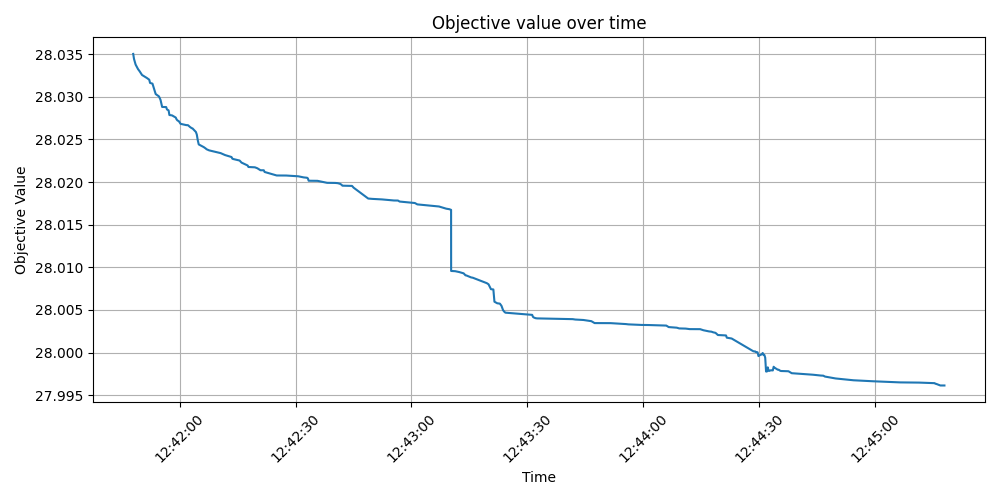
\includegraphics[width=1.0\textwidth]{figures/objective.png}
%% Use \caption command for figure caption and label.
\caption{Figure Caption}\label{fig:response-to-inclusion}
%% https://en.wikibooks.org/wiki/LaTeX/Importing_Graphics#Importing_external_graphics
\end{figure}

\subsection{Response to Exclusion}
\begin{figure}[H]%% placement specifier
%% Use \includegraphics command to insert graphic files. Place graphics files in 
%% working directory.
\centering%% For centre alignment of image.
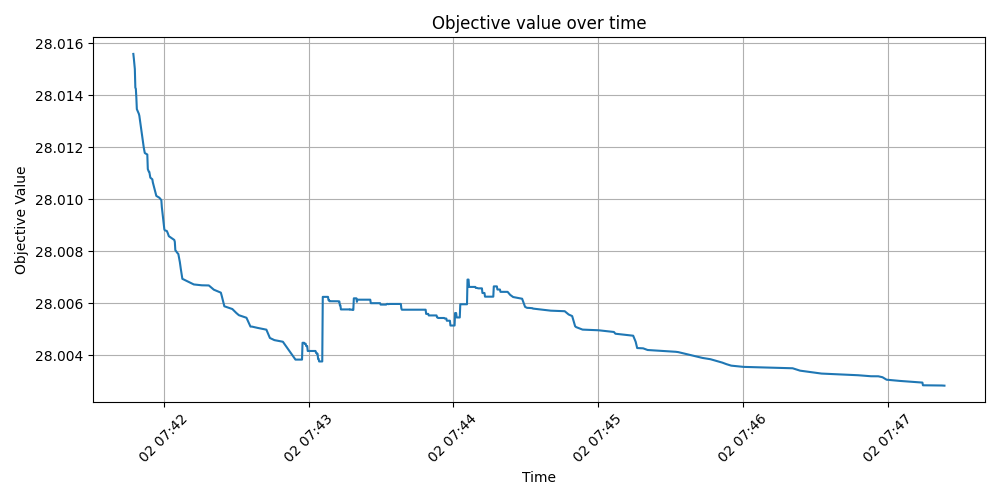
\includegraphics[width=1.0\textwidth]{figures/objective-400-exclusions.png}
%% Use \caption command for figure caption and label.
\caption{Figure Caption}\label{fig:objective-exclusion-400}
%% https://en.wikibooks.org/wiki/LaTeX/Importing_Graphics#Importing_external_graphics
\end{figure}

\subsection{Response to Changes in Knapsack Capacities}
The effects of changes to capacities will be illustrated in the same way as it was with the response to inclusion and below we see the table that shows which inputs that the AbLNS will be affected by.

\begin{table}[H]
\centering
\begin{tabular}{|c|c|c|c|c|c|}
\hline
                      & \begin{tabular}[c]{@{}c@{}}At Time:\\ 01:00\end{tabular} & \begin{tabular}[c]{@{}c@{}}At Time:\\ 02:00\end{tabular} & \begin{tabular}[c]{@{}c@{}}At Time:\\ 03:00\end{tabular} & \begin{tabular}[c]{@{}c@{}}At Time:\\ 04:00\end{tabular} & \begin{tabular}[c]{@{}c@{}}At Time:\\ 05:00\end{tabular} \\ \hline
$\Delta |p|$ & 16                                                       & 16                                                       & 16                                                       & 16                                                       & 16                                                       \\ \hline
$\Delta |\tau|$ & 16                                                       & 16                                                       & 16                                                       & 16                                                       & 16                                                       \\ \hline
$\Delta |cap|$& 100                                                      & 200                                                      & 400                                                      & 800                                                      & 1600                                                     \\ \hline
\end{tabular}
\end{table}

\begin{figure}[H]%% placement specifier
%% Use \includegraphics command to insert graphic files. Place graphics files in 
%% working directory.
\centering%% For centre alignment of image.
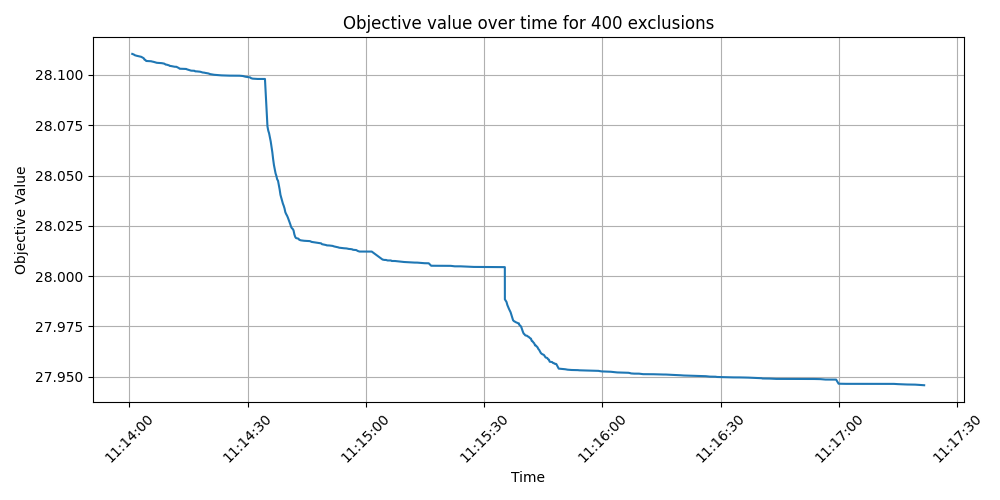
\includegraphics[width=1.0\textwidth]{figures/objective-resource-increases.png}
%% Use \caption command for figure caption and label.
\caption{Figure Caption}\label{fig:objective-resource-increases}
%% https://en.wikibooks.org/wiki/LaTeX/Importing_Graphics#Importing_external_graphics
\end{figure}

Correspondingly we also have the figure below in which the resources are decreasing.

\subsection{Response to Changes in Item Weights}
The final parameter that will be changed is the work order value $v$. This section will be more elaborate as we have to show how that the
work orders are rearranged due to the changes in their value across the different periods.

\begin{table}[H]
\centering
\begin{tabular}{|c|c|c|c|c|c|}
\hline
             & \begin{tabular}[c]{@{}c@{}}At Time:\\ 01:00\end{tabular} & \begin{tabular}[c]{@{}c@{}}At Time:\\ 02:00\end{tabular} & \begin{tabular}[c]{@{}c@{}}At Time:\\ 03:00\end{tabular} & \begin{tabular}[c]{@{}c@{}}At Time:\\ 04:00\end{tabular} & \begin{tabular}[c]{@{}c@{}}At Time:\\ 05:00\end{tabular} \\ \hline
$\Delta |w|$ & 20                                                       & 40                                                       & 80                                                       & 160                                                      & 320                                                      \\ \hline
$\Delta |p|$ & 26                                                       & 26                                                       & 26                                                       & 26                                                       & 26                                                       \\ \hline
$\Delta |v|$ & $1 \cdot 10^{5}$                                         & $2 \cdot 10^{5}$                                         & $4 \cdot 10^{5}$                                         & $8 \cdot 10^{5}$                                         & $1.6 \cdot 10^{6}$                                       \\ \hline
\end{tabular}
\end{table}

